\documentclass{article}
\usepackage{eecstex}
\usepackage{pgfplots}
\usepackage{physics}

\DeclareMathOperator{\rect}{rect}

\title{Homework 1}
\author{Bryan Ngo}
\date{2022-01-19}

\begin{document}

\maketitle

\setcounter{section}{1}

\section{}

\subsection{}

\begin{theorem}
    The system \(L\) is not time invariant.
\end{theorem}
\begin{proof}
    We can represent a time-delayed signal as a linear combination of the other 3 signals.
    We can represent the 3 input signals in a matrix
    \begin{equation}
        \bm{X} =
        \begin{bmatrix}
           -2 & -2 & 0 \\
           1 & 1 & 1 \\
           -2 & 0 & 1 
        \end{bmatrix}
    \end{equation}
    Then, we can find the linear combination necessary to create a time delayed signal (for example, \(x_2[n - 1]\)) by solving the system of equations
    \begin{equation}
        \bm{Xa} =
        \begin{bmatrix}
            0 \\
            -2 \\
            1
        \end{bmatrix}
    \end{equation}
    where we get \(\bm{a} = \begin{bmatrix}
        -\frac{3}{2} & \frac{3}{2} & -2
    \end{bmatrix}^\top\).
    Thus, we have
    \begin{equation}
        x_2[n - 1] = -\frac{3}{2} x_1[n] + \frac{3}{2} x_2[n] - 2x_3[n]
    \end{equation}
    Calculating \(-\frac{3}{2} y_1[n] + \frac{3}{2} y_2[n] - 2y_3[n]\),
    we get the following plot:
    \begin{center}
        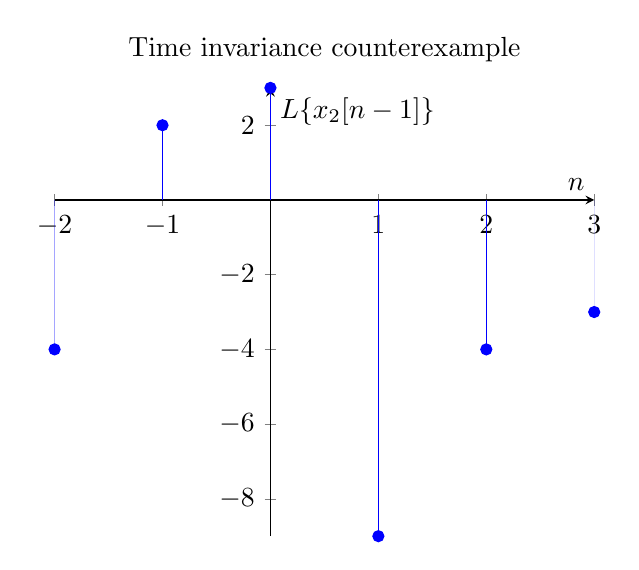
\begin{tikzpicture}
            \begin{axis}[
                xlabel=\(n\), ylabel={\(L\{x_2[n - 1]\}\)},
                title={Time invariance counterexample},
                axis lines=middle
            ]
            \addplot[
                ycomb,
                color=blue,
                mark=*
            ]
            coordinates {
                (-2, -4)
                (-1, 2)
                (0, 3)
                (1, -9)
                (2, -4)
                (3, -3)
            };
            \end{axis}
        \end{tikzpicture}
        \begin{tikzpicture}
            \begin{axis}[
                xlabel=\(n\), ylabel={\(y_2[n - 1]\)},
                title={Expected output signal},
                axis lines=middle
            ]
            \addplot[
                ycomb,
                color=blue,
                mark=*
            ]
            coordinates {
                (0, -1)
                (1, 1)
                (2, -3)
                (3, -0)
                (4, -1)
            };
            \end{axis}
        \end{tikzpicture}
    \end{center}
    So the system is \emph{not} time-invariant.
\end{proof}

\subsection{}

We can represent the delta function as
\begin{equation}
    \delta[n] = \frac{1}{2} (x_1[n] - x_2[n] + 2x_3[n])
\end{equation}
Using the properties of linear systems, we can find the impulse response
\begin{equation}
    h[n] = \frac{1}{2} (y_1[n] - y_2[n] + 2y_3[n])
\end{equation}
which gives us the following plot:
\begin{center}
    \begin{tikzpicture}
        \begin{axis}[
            xlabel=\(n\), ylabel={\(L\{\delta[n]\}\)},
            title={Impulse response},
            axis lines=middle
        ]
        \addplot[
            ycomb,
            color=blue,
            mark=*
        ]
        coordinates {
            (-2, 2)
            (-1, 1)
            (0, -2)
            (1, 3)
            (2, 2)
            (3, 1)
        };
        \end{axis}
    \end{tikzpicture}
\end{center}

\section{}

\begin{align}
    y[n] - ay[n - 1] &= x[n] \\
    y[0] &= 1
\end{align}

\subsection{}

For the homogenuous solution, assume that \(y_h[n] = A\lambda^n\).
Then,
\begin{align}
    A\lambda^n - aA\lambda^{n - 1} &= 0 \\
    1 - a\lambda^{-1} &= 0 \\
    \implies \lambda &= a
    \implies y_h[n] = Aa^n
\end{align}
Finding the particular solution,
\begin{equation}
    \begin{array}[]{||c|c||}
        \hline
        n & x[n] \\
        \hline
        0 & 1 \\
        1 & x[1] + a = y[1] \\
        2 & x[2] + a x[1] + a^2 = y[2] \\
        3 & x[3] + a x[2] + a^2 x[1] = y[3] \\
        \vdots & \vdots \\
        \hline
    \end{array}
\end{equation}

%% TODO: fix this

\subsection{}

\subsection{}

\section{}

\begin{equation}
    y[n] = h[n] \ast (\cos[\omega_0 n] x[n]) = \sum_{k \geqslant 0} \frac{1}{1 + k} \cos[\omega_0 (n - k)] x[n - k]
\end{equation}

\subsection{}

\begin{theorem}
    The above system is not LTI.
\end{theorem}
\begin{proof}
    Proving linearity, suppose we are given the system responses \(x_1[n] \iff y_1[n]\) and \(x_2[n] \iff y_2[n]\),
    \begin{align}
        T\{a x_1[n] + b x_2[n]\} &= \sum_{k \geqslant 0} \frac{1}{1 + k} \cos[\omega_0 n] (a x_1[n - k] + b x_2[n - k]) \\
        &= a \sum_{k \geqslant 0} \frac{1}{1 + k} \cos[\omega_0 n] x_1[n - k] + b \sum_{k \geqslant 0} \frac{1}{1 + k} \cos[\omega_0 n] x_2[n - k] \\
        &= a y_1[n] + b y_2[n]
    \end{align}
    Consider the inputs \(x[n] = \delta[n]\) and \(n_0 = 1\),
    \begin{align}
        T\{\delta[n]\} &= h[n] \ast (\cos[\omega_0 n] \delta[n]) =
        \begin{cases}
            0 & n < 0 \\
            \frac{1}{1 + n} \cos[\omega_0 n] & n \geqslant 0
        \end{cases} \\
        T\{\delta[n - 1]\} &= h[n - 1] \ast (\cos[\omega_0 n - \omega_0] \delta[n - 1]) \\
        &= h[n - 2] \cos[\omega_0 n - \omega_0] =
        \begin{cases}
            0 & n < 2 \\
            \frac{1}{n - 1} \cos[\omega_0 n - \omega_0] & n \geqslant 2
        \end{cases} \neq y[n - 1] \\
    \end{align}
\end{proof}

\subsection{}

The system is not BIBO stable, since if \(|x[n]| < B_x\), then
\begin{equation}
    |y[n]| = \sum_{k \geqslant 0} \frac{1}{1 + k} B_x \not< \infty
\end{equation}
due to the divergence of the harmonic series.

\subsection{}

The system is causal, since the summation in the convolution with \(h[n]\) only relies on past values of \(x[n]\).

\section{}

\subsection{}

We can model the frequency response as
\begin{equation}
    H(e^{j \omega}) = \rect\left(\frac{\omega}{\pi}\right)
\end{equation}
Finding the inverse Fourier transform,
\begin{align}
    h[n] &= \frac{1}{2\pi} \int_{-\pi}^\pi H(e^{j \omega}) e^{j \omega n} \, d\omega \\
    &= \frac{1}{2\pi} \int_{-\frac{\pi}{2}}^{\frac{\pi}{2}} e^{j \omega n} \, d\omega = \frac{1}{2\pi} \eval{\frac{e^{j \omega n}}{jn}}_{-\frac{\pi}{2}}^{\frac{\pi}{2}} \\
    &= \frac{1}{2\pi j n} \left(e^{j \frac{\pi}{2} n} - e^{-j \frac{\pi}{2} n}\right) = \frac{\sin\left[\frac{\pi}{2} n\right]}{\pi n}
\end{align}

\subsection{}

The system is not causal, since \(h[-1] = \frac{1}{\pi} \neq 0\).

\subsection{}

\begin{equation}
    \begin{array}[]{||c|c||}
        \hline
        n & h[n] \\
        \hline
        0 & \frac{1}{\pi} \\
        1 & \frac{1}{\pi} \\
        3 & -\frac{1}{3\pi} \\
        5 & \frac{1}{5\pi} \\
        \vdots & \vdots \\
        \hline
    \end{array}
\end{equation}
The system is BIBO stable, since
\begin{equation}
    \sum_{k = -\infty}^\infty |h[k]| = \frac{1}{\pi} + \frac{2}{\pi} \underbrace{\left(1 - \frac{1}{3} + \frac{1}{5} - \frac{1}{7} + \cdots\right)}_{\frac{\pi}{4}} = \frac{1}{\pi} + \frac{1}{2} < \infty
\end{equation}
where we use the evenness of the sinc function and the Leibniz formula for \(\pi\).

%% TODO: probably not BIBO stable

\section{}

\begin{equation}
    y[n] = \frac{1}{6} \sum_{k = 0}^5 x[n - k]
\end{equation}

\subsection{}

\begin{align}
    T\{e^{j \omega n}\} &= \frac{1}{6} \sum_{k = 0}^5 e^{j \omega (n - k)} \\
    &= \frac{1}{6} \sum_{k = 0}^5 e^{j \omega n} e^{-j \omega k} = e^{j \omega n} \left(\frac{1}{6} \sum_{k = 0}^5 e^{-j \omega k}\right) \\
    \implies H(e^{j \omega}) &= \frac{1}{6} \sum_{k = 0}^5 e^{-j \omega k}
\end{align}
Using Equation 2.123 from Oppenheim \& Schafer with \(M_2 = 5\),
\begin{align}
    H(e^{j \omega}) &= \frac{1}{6} \frac{\sin(3\omega)}{\sin\left(\frac{\omega}{2}\right)} e^{-j \frac{5}{2} \omega} \\
    |H(e^{j \omega})| &= \frac{1}{6} \left|\frac{\sin(3\omega)}{\sin\left(\frac{\omega}{2}\right)}\right| \\
    \angle H(e^{j \omega}) &= \angle \sin(3 \omega) - \angle \sin\left(\frac{\omega}{2}\right) - \frac{5}{2} \omega
\end{align}
The zero crossings are \(\omega = \frac{k\pi}{3}\) for \(k \in \Z\).
\begin{center}
    \begin{tikzpicture}
        \begin{axis}[
            xlabel=\(\omega\), ylabel={\(|H(e^{j \omega})|\)},
            title={Magnitude of Frequency Response},
            axis lines=middle,
            ymin=0, ymax=1,
            width=0.4\textwidth
        ]
        \addplot[color=blue] table[
            col sep=comma,
            x=n, y=q6a-mag
        ]{q6a-mag.csv};
        \end{axis}
    \end{tikzpicture}
\end{center}

\end{document}
